
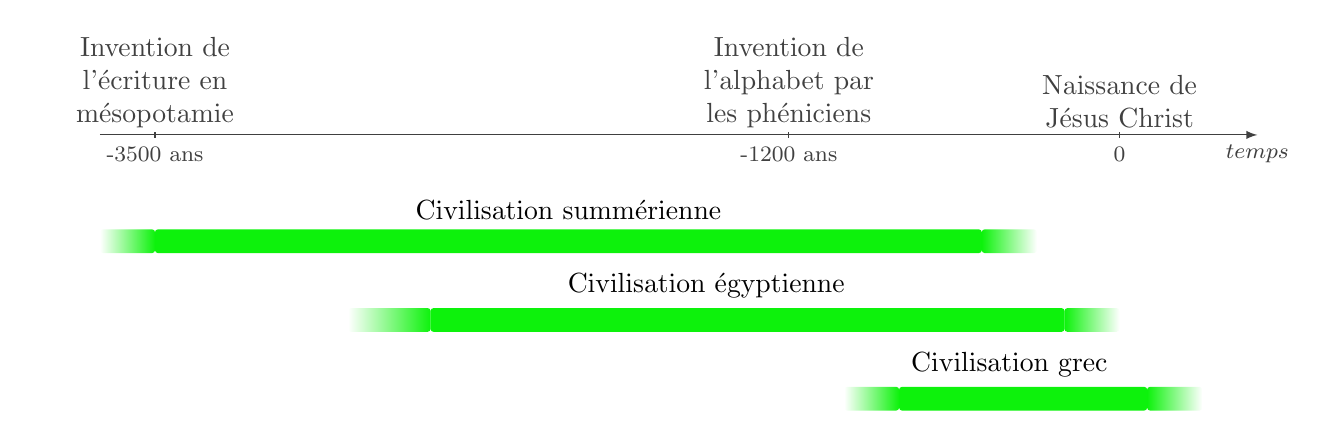
\begin{tikzpicture}
    \def\horizontal {0.35}
    \def\vertical {1.3}
\begin{scope}
\draw[-latex,color=darkgray] (-37*\horizontal,0) -- (5*\horizontal,0);
\draw[shift={(5*\horizontal,0)},color=darkgray,thin]
                                   node[below] {\footnotesize $temps$};
%3500 av JC
  \draw[shift={(-35*\horizontal,0)},color=darkgray,thin] (0pt,1pt) -- (0pt,-1pt)
                                   node[above,text width=3cm,text centered]{ Invention de l'écriture en mésopotamie}
                                   node[below] {\footnotesize -3500 ans};
%776 av JC
  \draw[shift={(-12*\horizontal,0)},color=darkgray,thin] (0pt,1pt) -- (0pt,-1pt)
                                   node[above,text width=3cm,text centered]{ Invention de l'alphabet par les phéniciens}
                                   node[below] {\footnotesize -1200 ans};
  \draw[shift={(0,0)},color=darkgray,thin] (0pt,1pt) -- (0pt,-1pt)
                                   node[below] {\footnotesize 0}
                                   node[above,text width=3cm,text centered]{ Naissance de Jésus Christ};
%\draw (1.4*\horizontal,0.5*\vertical) node [rotate=30]{Ptolémé};
\end{scope}
\begin{scope}[yshift= -1.5cm]
    \def\vertical {0.3}
  \shade[bottom color=brown!10!gray!10!green, top color=white,shading angle={90},rounded corners=1pt]
 (-37*\horizontal,0) rectangle (-35*\horizontal, \vertical);
  \shade[bottom color=brown!10!gray!10!green, top color=brown!10!gray!10!green,shading angle={90},rounded corners=1pt]
 (-35*\horizontal,0) rectangle (-5*\horizontal, \vertical);
  \shade[bottom color=white, top color=brown!10!gray!10!green,shading angle={90},rounded corners=1pt]
 (-5*\horizontal,0) rectangle (-3*\horizontal, \vertical);
  \node[above] (P) at (-20*\horizontal,\vertical) {Civilisation summérienne}; % SUMÉRIENS

    \def\decalage {-1}
  \shade[bottom color=brown!10!gray!10!green, top color=white,shading angle={90},rounded corners=1pt]
 (-28*\horizontal, \decalage) rectangle (-25*\horizontal, \vertical + \decalage);
  \shade[bottom color=brown!10!gray!10!green, top color=brown!10!gray!10!green,shading angle={90},rounded corners=1pt]
 (-25*\horizontal, \decalage) rectangle (-2*\horizontal, \vertical + \decalage);
  \shade[bottom color=white, top color=brown!10!gray!10!green,shading angle={90},rounded corners=1pt]
 (-2*\horizontal, \decalage) rectangle (0*\horizontal, \vertical + \decalage);
  \node[above] (P) at (-15*\horizontal,\vertical  + \decalage) {Civilisation égyptienne}; % ÉGYPTIENS

    \def\decalage {-2}
  \shade[bottom color=brown!10!gray!10!green, top color=white,shading angle={90},rounded corners=1pt]
 (-10*\horizontal, \decalage) rectangle (-8*\horizontal, \vertical + \decalage);
  \shade[bottom color=brown!10!gray!10!green, top color=brown!10!gray!10!green,shading angle={90},rounded corners=1pt]
 (-8*\horizontal, \decalage) rectangle (1*\horizontal, \vertical + \decalage);
  \shade[bottom color=white, top color=brown!10!gray!10!green,shading angle={90},rounded corners=1pt]
 (1*\horizontal, \decalage) rectangle (3*\horizontal, \vertical + \decalage);
  \node[above] (P) at (-4*\horizontal,\vertical  + \decalage) {Civilisation grec}; % CRECS
\end{scope}
\end{tikzpicture}


%%%%%%%%%%%%%%%%%%%%%%%%%%%%%%%%%%%%%%%%%%%



